\appendix
\section{Appendix}
\subsection{Matching Procedure Justification}
The treatment effect after matching can be calculated as in Equation \ref{eq:1te}, where $\hat{\alpha}$ is the estimated treatment effect, $T$ is the set of treated observations, $C$ that of the controls. $Y_{it}$ is the outcome value of interest for observation $i$ at time $t$. $w_j$ is the weight assigned to each control observation. In matching without replacement and without ties this would be either one or zero. In matching with replacement and or ties this can be any real value larger than zero. These weights sum up to the number of treated observations.
\begin{equation} \label{eq:1te}
    \hat{\alpha} = \sum_{i \in T} \Delta Y_{i, 15} - \sum_{j \in C} w_j \Delta Y_{j,15}
\end{equation}

In line with synthetic control method studies (e.g. \citealp{Abadie2006, Dube2015}), we assume $Y_{it}$ can be modeled in a multi factor error structure (see e.g. \citealp{Chudik2015, Bai2009}) as in Equation \ref{eq:2mfs}. $\alpha_i$ is the firm-specific treatment effect, $D_t$ is one from 2015 onwards and zero before, I(..) indicates whether the firm is treated. $c_i$ is a firm-specific fixed effect, $\delta_t$ is a period specific common shock and $\epsilon_{it}$ is a mean zero (time-varying) idiosyncratic shock. $F_t$ is a time-varying economy wide shock that affects each firm differently, according to their specific factor loading $\lambda_i$. There can be a potentially large number of these, but for ease of exposition we stick to one.

\begin{equation}\label{eq:2mfs}
    Y_{it} = \alpha_i D_t I(i \in T) + c_i + \delta_t + F_t \lambda_i + \epsilon_{it}
\end{equation}

Substituting in our model for $Y_it$ and expanding the difference operator leads to Equation \ref{eq:3fullte}.

\begin{equation}\label{eq:3fullte}
    \begin{split}
         \hat{\alpha} =\sum_{i \in T} \alpha_i + &(c_i - c_i) + (\delta_{15} - \delta_{14}) + \lambda_i * (F_{15} - F_{14}) + (\epsilon_{i,15} - \epsilon_{i,14})  \\
         - \sum_{j \in C} w_j [ &(c_j - c_j) + (\delta_{15} - \delta_{14}) + \lambda_j * (F_{15} - F_{14}) + (\epsilon_{j,15} - \epsilon_{j,14})]
    \end{split}
\end{equation}

The $c$'s drop out due to the time differing. Given that $\sum_{i \ in T}1 = \sum_{j \in C} w_j$, the deltas in treated and control also cancel out eachother. The $\epsilon$'s are assumed to be mean zero, so as $T$ and $C$ get large, these also drop out, leaving us with Equation \ref{eq:4reducedte}.

\begin{align}\label{eq:4reducedte}
         \hat{\alpha} &=\sum_{i \in T} \alpha_i + \lambda_i * (F_{15} - F_{14}) 
         - \sum_{j \in C} w_j \lambda_j * (F_{15} - F_{14}) \nonumber\\
                     &=\sum_{i \in T} \alpha_i + \bigg(\sum_{i \in T}\lambda_i - \sum_{j \in C} w_j \lambda_j\bigg) * (F_{15} - F_{14})
\end{align}

The remaining bias terms are a function of the disparity in the treated and untreated factor loadings $\lambda$. This is where the synthetic control method intuition comes in: if we match on pretreatment outcome values, then as $T$, $C$ and the number of pretreatment periods we match on get larger, the average difference between treated and untreated factor loadings $\lambda$ goes to zero. The idea is that with just one pretreatment period you might still be able to find a set of weights $w_j$ such that treated and untreated firms with different factor loadings match due to compensating idiosyncratic $\epsilon$'s. As the pretreatment period becomes longer, this becomes increasingly unlikely (given time constant weights). Instead, this only remains possible if your matching algorithm achieved matches by picking controls firms such that the weighted sum of their factor loadings $\sum_{j \in C} w_j \lambda_j$ equals the sum of the treated factor loadings $\sum_{i \in T}\lambda_i$. Under that assumption, Equation \ref{eq:4reducedte} reduces to Equation \ref{eq:5success}, where all bias terms have been accounted for.

\begin{equation}\label{eq:5success}
    \hat{\alpha} = \sum_{i \in T}\alpha_i
\end{equation}


% Replication: ctrl+F #sectorBiteTable
\begin{table}[htbp]\centering
%\setlength\tabcolsep{3pt}
\tiny
\caption{Overview of bite, gap and wage bill indicators by sector (East-West)}\label{table:sectorBite}
\begin{threeparttable}
    \begin{tabular}{r|c|c|c|l}
    \toprule
Nace & Share    & Gap       & Wage Bill     & Nace  \\
Code & West-East& West-East & West-East     & Text \\
\midrule
55&	52 - 64&	1.37 - 2.14&	12 - 26&	Accommodation\\
56&	52 - 64&	1.36 - 2.13&	12 - 26&	Food and beverage service activities\\
47&	29 - 48&	0.70 - 1.26&	4 - 12&	Retail trade, excl. of motor vehicles and motorcycles\\
69&	23 - 45&	0.49 - 0.99&	2 - 7&	Legal and accounting activities\\
12&	23 - 45&	0.49 - 0.99&	2 - 7&	Manufacture of tobacco products\\
80&	23 - 44&	0.48 - 0.97&	2 - 7&	Security and investigation activities\\
73&	23 - 44&	0.48 - 0.98&	2 - 7&	Advertising and market research\\
78&	23 - 44&	0.48 - 0.98&	2 - 7&	Employment activities\\
74&	23 - 43&	0.48 - 0.97&	2 - 6&	Other professional, scientific and technical activities\\
71&	22 - 43&	0.47 - 0.96&	2 - 6&	Architectural and engineering activities; technical testing and analysis\\
11&	28 - 42&	0.52 - 0.94&	3 - 9&	Manufacture of beverages\\
45&	21 - 42&	0.53 - 1.20&	3 - 12&	Wholesale and retail trade and repair of motor vehicles and motorcycles\\
10&	28 - 42&	0.52 - 0.95&	3 - 9&	Manufacture of food products\\
70&	22 - 42&	0.47 - 0.95&	2 - 6&	Activities of head offices; management consultancy activities\\
82&	22 - 42&	0.47 - 0.94&	2 - 6&	Admin, office support and other business support activities\\
79&	16 - 41&	0.30 - 0.94&	2 - 8&	Travel agency, tour operator and related activities\\
52&	16 - 40&	0.30 - 0.93&	2 - 8&	Warehousing and support activities for transportation\\
77&	21 - 40&	0.46 - 0.91&	2 - 7&	Rental and leasing activities\\
50&	16 - 39&	0.31 - 0.87&	2 - 7&	Water transport\\
15&	20 - 39&	0.51 - 0.85&	3 - 9&	Manufacture of leather and related products\\
66&	11 - 38&	0.18 - 0.86&	0 - 6&	Activities auxiliary to financial services and insurance activities\\
14&	20 - 38&	0.63 - 0.82&	3 - 9&	Manufacture of wearing apparel\\
23&	12 - 38&	0.30 - 0.62&	2 - 5&	Manufacture of other non-metallic mineral products\\
95&	22 - 38&	0.53 - 0.99&	3 - 9&	Repair of computers and personal and household goods\\
13&	16 - 38&	0.27 - 0.77&	2 - 8&	Manufacture of textiles\\
63&	21 - 37&	0.47 - 0.88&	2 - 6&	Information service activities\\
51&	3 - 37&	0.06 - 0.89&	0 - 8&	Air transport\\
31&	14 - 34&	0.33 - 0.35&	2 - 4&	Manufacture of furniture\\
68&	14 - 32&	0.32 - 0.87&	1 - 5&	Real estate activities\\
93&	26 - 32&	0.73 - 0.93&	5 - 8&	Sports activities and amusement and recreation activities\\
19&	12 - 29&	0.29 - 0.43&	2 - 4&	Manufacture of coke and refined petroleum products\\
8&	14 - 29&	0.32 - 0.61&	2 - 5&	Other mining and quarrying\\
61&	23 - 29&	0.60 - 0.92&	2 - 6&	Telecommunications\\
49&	21 - 28&	0.47 - 0.66&	2 - 5&	Land transport and transport via pipelines\\
91&	23 - 28&	0.67 - 0.84&	4 - 6&	Libraries, archives, museums and other cultural activities\\
60&	23 - 28&	0.67 - 0.85&	4 - 6&	Programming and broadcasting activities\\
92&	23 - 28&	0.67 - 0.85&	4 - 6&	Gambling and betting activities\\
59&	22 - 28&	0.64 - 0.82&	3 - 6&	Audiovisual productions\\
90&	23 - 28&	0.67 - 0.85&	4 - 6&	Creative, arts and entertainment activities\\
53&	23 - 28&	0.61 - 0.93&	2 - 6&	Postal and courier activities\\
94&	11 - 26&	0.20 - 0.58&	1 - 3&	Activities of membership organisations\\
18&	15 - 26&	0.40 - 0.53&	1 - 4&	Printing and reproduction of recorded media\\
87&	14 - 26&	0.27 - 0.49&	1 - 3&	Residential care activities\\
75&	14 - 26&	0.27 - 0.49&	1 - 3&	Veterinary activities\\
58&	15 - 26&	0.40 - 0.54&	1 - 4&	Publishing activities\\
88&	14 - 26&	0.27 - 0.50&	1 - 3&	Social work activities without accommodation\\
17&	10 - 26&	0.27 - 0.48&	1 - 4&	Manufacture of paper and paper products\\
86&	14 - 26&	0.27 - 0.49&	1 - 3&	Human health activities\\
42&	7 - 23&	0.20 - 0.45&	1 - 4&	Civil engineering\\
41&	8 - 23&	0.21 - 0.48&	1 - 4&	Construction of buildings\\
16&	13 - 23&	0.38 - 0.19&	2 - 2&	Manufacture of wood related products, straw and plaiting, excl. furniture\\
46&	12 - 22&	0.21 - 0.21&	1 - 2&	Wholesale trade, excl. of motor vehicles and motorcycles\\
30&	8 - 22&	0.12 - 0.38&	0 - 3&	Manufacture of other transport equipment\\
32&	8 - 22&	0.16 - 0.20&	1 - 2&	Other manufacturing\\
22&	12 - 22&	0.27 - 0.45&	1 - 4&	Manufacture of rubber and plastic products\\
43&	7 - 22&	0.20 - 0.44&	1 - 4&	Specialised construction activities\\
29&	5 - 22&	0.09 - 0.44&	0 - 3&	Manufacture of motor vehicles, trailers and semi-trailers\\
6&	5 - 21&	0.12 - 0.30&	1 - 2&	Extraction of crude petroleum and natural gas\\
72&	10 - 21&	0.29 - 0.42&	1 - 3&	Scientific research and development \\
24&	3 - 20&	0.05 - 0.31&	0 - 2&	Manufacture of basic metals\\
25&	6 - 20&	0.12 - 0.30&	1 - 2&	Manufacture of fabricated metal products, excl. machinery and equipment\\
33&	7 - 18&	0.14 - 0.28&	1 - 2&	Repair and installation of machinery and equipment\\
26&	6 - 17&	0.12 - 0.20&	0 - 1&	Manufacture of computer, electronic and optical products\\
27&	5 - 16&	0.10 - 0.32&	0 - 2&	Manufacture of electrical equipment\\
65&	7 - 15&	0.16 - 0.54&	0 - 3&	(re-)Insurance and pension funding, excl. compulsory social security\\
5&	4 - 13&	0.11 - 0.23&	1 - 2&	Mining of coal and lignite\\
62&	6 - 13&	0.17 - 0.47&	1 - 2&	Computer programming, consultancy and related activities\\
9&	5 - 12&	0.12 - 0.21&	0 - 2&	Mining support service activities\\
21&	3 - 12&	0.06 - 0.21&	0 - 1&	Manufacture of basic pharmaceutical products and preparations\\
20&	3 - 12&	0.05 - 0.21&	0 - 1&	Manufacture of chemicals and chemical products\\
36&	7 - 11&	0.16 - 0.28&	1 - 2&	Water collection, treatment and supply\\
28&	3 - 10&	0.08 - 0.14&	0 - 1&	Manufacture of machinery and equipment n.e.c.\\
85&	11 - 9&	0.26 - 0.24&	1 - 1&	Education\\
39&	7 - 9&	0.15 - 0.17&	1 - 1&	Remediation activities and other waste management services\\
35&	5 - 8&	0.12 - 0.21&	0 - 1&	Electricity, gas, steam and air conditioning supply\\
37&	6 - 7&	0.14 - 0.14&	1 - 1&	Sewerage\\
64&	3 - 7&	0.07 - 0.08&	0 - 0&	Financial service activities, excl. insurance and pension funding\\
38&	6 - 6&	0.13 - 0.12&	1 - 1&	Waste collection, treatment and disposal activities; materials recovery\\
84&	4 - 5&	0.08 - 0.16&	0 - 1&	Public administration and defence; compulsory social security\\
    \bottomrule
    \end{tabular}
\begin{tablenotes}
\item \footnotesize Unlisted sectors are excluded based on legislative reasons or due to pre-existing higher sectoral minimum wage agreements. \emph{Share}: share earning less than 8.50 in 2013-2014 (percentage). \emph{Gap}: gap between hourly wage in 2013-2014 and MW for those earning less than the MW. \emph{Wage Bill}: relative increase in total wage bill under full compliance and no spillovers (percentage).
\end{tablenotes}
\end{threeparttable}
\end{table}

% Replication: ctrl+F #correlationIndicatorsGraph
\begin{figure}[htbp]
    \centering
    \caption{Correlation share, gap and wage bill indicators}
    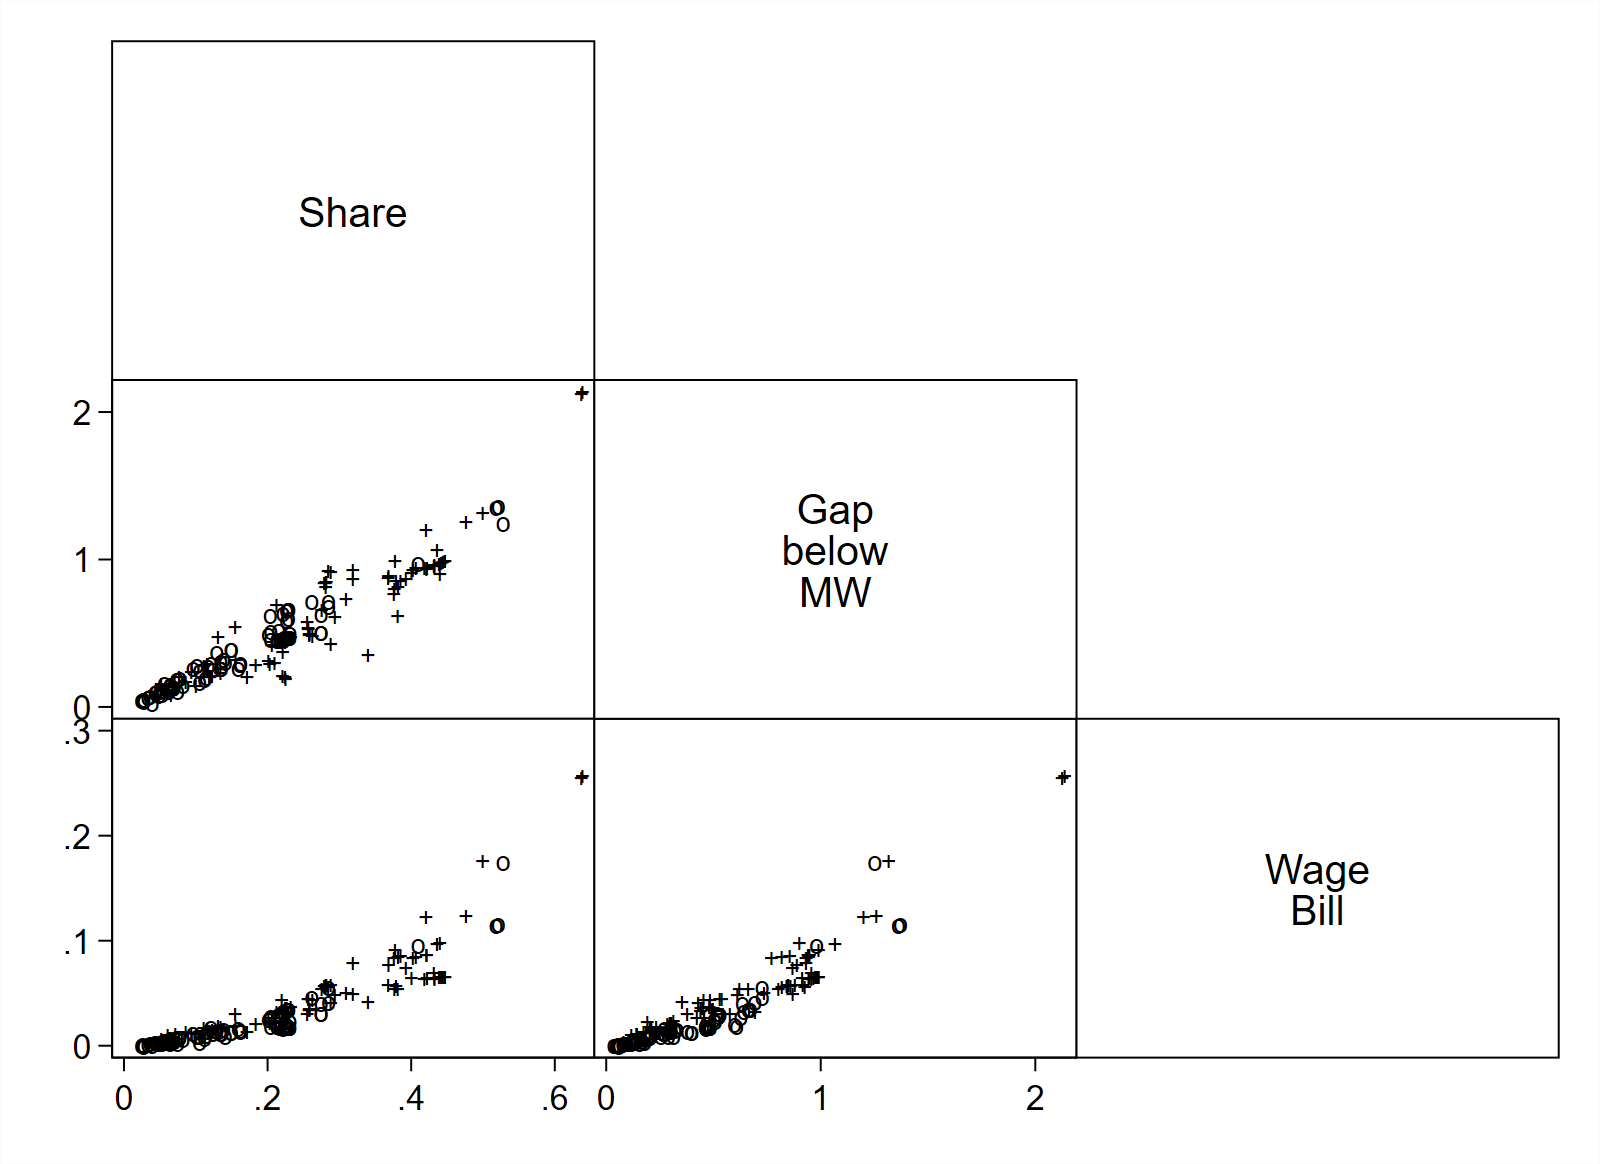
\includegraphics[width=0.70\paperwidth]{Images/shareGapWbi.png}
    \label{fig:correlationIndicators}
    \caption*{See notes below Table \ref{table:sectorBite} for a description of the indicators. +: values for sectors in the East, o: the West.}
\end{figure}

% Tw Results
% Replication: ctrl+F #twResultsTable
\begin{table}[htbp]\centering
\caption{Employment and Turnover Effects - Smaller Grey Zone}\label{table:twResults}
\begin{threeparttable}
\begin{tabular}{l|cc|cc}
\toprule
&\multicolumn{2}{c|}{East}&\multicolumn{2}{c}{West}\\
&Emp&Turn & Emp&Turn\\
&(1)&(2)&(3)&(4)\\
\midrule
$\Delta$ Growth 14-15 &-.002& 0& 0 & -.003\\
&(.002)& (.003)& (.002) & (.002) \\
$\Delta$ Growth 14-16 &-.006& 0& -.001 & -.005\\
&(.003)\sym{**}& (.004)& (.002) & (.003) \\
\midrule
\# of treated &7256& 5168& 12164 & 8688\\
\# of controls &66176& 47280& 66176 & 47281\\
\# of controls used &13328& 4730& 19250 & 7914\\
\midrule
SDM 13-14 &.03& 0& .01& -.01\\  % Note: East-Emp 1314 SDM exceeds point estimate SDM 
Level Diff 2013&0& -.01& 0& 0\\
Trend 2011-2014&\checkmark&\checkmark&\checkmark&\checkmark \\
Specification & Base & Prod & Base & Base\\
\bottomrule
\end{tabular}
\begin{tablenotes}
\item $\Delta$ Growth is the difference in growth between the treated and control. SDM refers to the standardised difference in means. 
Level Diff 2013 indicates the difference in log levels between treated and control in 2013. 
Trend indicates how this level difference evolved between 2011 and 2014.
Specification shows which matching specification scored best at the evaluation criteria. Prod: match also on 2014 labour productivity of firm (emp/turn).
\item Matching uncertainty robust AI standard errors in parentheses \citep{Abadie2006}.
\item \emph{Stars}: \sym{*} \(p<0.1\), \sym{**} \(p<0.05\), \sym{***} \(p<0.01\)
\end{tablenotes}
\end{threeparttable}
\end{table}